
\section{Artificial Neural Networks (ANN)}
An ANN is a data-structure to define arbitrarily complex mathematical functions

\subsection{Artificial Neurons}
\begin{itemize}
    \item Receives an input vector $[x_1,x_2, ...]$
    \item Each neuron has its own input weights $[w_1, w_2, ...]$ and \textcolor{blue}{bias} b (=intercept)
    \item Calculates the sum of the weighted input (dot product $\vec{x} * \vec{w}$), adds a bias b, and passes it through a nonlinear activation function
\end{itemize}
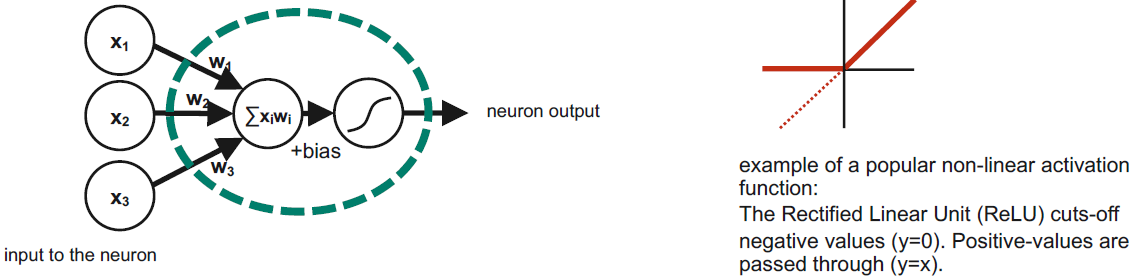
\includegraphics[width=\linewidth]{artificial_neurons.png}

\subsection{Simple Artificial Neural Network (ANN)}
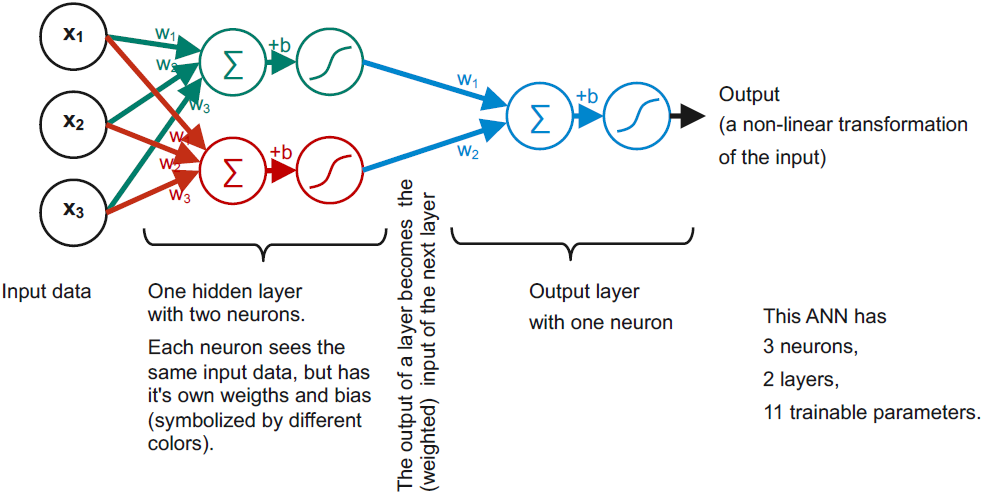
\includegraphics[width=\linewidth]{ann.png}

\subsection{Training an ANN}
\textbf{Supervised learning}
\begin{itemize}
    \item Data with label
    \item For each input $\vec{x}$ we are given the output $\vec{y}$
    \item ANN is initialized with random weights
    \item An optimizer reduces a cost-function (e.g. MSE)
    \item At every iteration, and for every single weight $w$ and bias $b$, the partial derivative needs to be calculated. (Backpropagation algorithm)
\end{itemize}
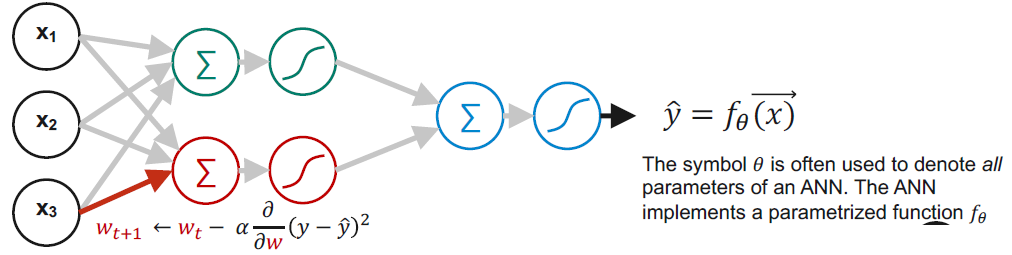
\includegraphics[width=\linewidth]{train_ann.png}
